\chapter{Konzept zur Visualisierung von Schmerz Scores aus akustischen Signalen}

Das in dieser Arbeit umzusetzende System muss den folgenden Anforderungen genügen:
\begin{enumerate}
	\item Das System muss dazu in der Lage sein, aus den akustischen Eigenschaften des Weinens eines Babys den Schmerz Score bezüglich einer Pain Scale abzuleiten.
	\item Das System muss dazu in der Lage sein, die abgeleiteten Schmerz Scores zu visualiseren.
	\item Das System muss dazu in der Lage sein, beliebige Pain Scales einzubinden. 
	\item Die System muss dazu in der Lage sein,  die Analyse auch bei nicht-optimalen akustischen Bedingungen durchzuführen.
	\item Das System muss dazu in der Lage sein, die Analyse kontinuierlich durchzuführen.
\end{enumerate}

\section{Literaturüberblick}
\label{sec:system_literature}

In diesem Kapitel wird ein Überblick über bereits veröffentlichte Ansätze zur Analyse akustischer Signale von Neugeborenen gegeben.

Ein großer Teil der Veröffentlichungen stellt Algorithmen zur Klassifizierung einzelner Cry Units vor, entweder bezüglich der Weinursache (Hunger, Angst, Schmerz, ... ) oder zur Diagnose bestimmter Krankheiten. Diese Methoden sind in den meisten Fällen nicht für die kontinuierliche Analyse geeignet, sondern haben das Ziel, eine gegebenen Cry-Unit mit einer möglichst hohen Genauigkeit bezüglich der Ursache zu klassifizieren. Probleme wie Hintergrundrauschen, Berechnungsaufwand oder kontextuelle Informationen spielen eine untergeordnete Rolle. Beispiele für solche Veröffentlichungen sind die von Abdulaziz et al. \cite{class_abdulaziz} oder Fuhr et al. \cite{comparisonOfLearning}.

Várallyay stellte in seiner Dissertation \glqq Analysis of the Infant Cry with Objective Methods\grqq{} \cite{cry_thesis} Methoden zur automatisierten Analyse kindlicher Lautäußerungen vor. Das primäre Ziel der Dissertation war die Erforschung der Unterschiede zwischen den Lautäußerungen gesunder und tauber Neugeborener. Die Algorithmen zur automatisierten Analyse der Audiosignale waren ein \glqq Nebenprodukt\grqq{} zur schnelleren Datenauswertung. Die Auswertung musste nicht kontinuierlich erfolgen. In der vorgestellten Verarbeitungspipeline wurde das Eingangssignal in Zeitfenster weniger Millisekunden zerlegt und jedes Fenster nach Entscheidungsregeln als \emph{stimmhaft} oder \emph{nicht stimmhaft} markiert. Die stimmhaften Signalfenster wurden zu \emph{Segmenten} zusammengefasst (welche in Kapitel \ref{sec:acousticModel} als Cry-Units bezeichnet werden). Auf Basis der Segmente wurden Auswertungen bezüglich des Zeitbereiches (Durchschnittliche Segmentlänge, Pausenlängen etc.), des Frequenzbereiches (Grund-Frequenz, Formanten-Frequenzen etc.) und des Melodieverlaufes angestellt. Analysiert wurden Audioaufnahmen von Babys mit einer Länge von 10 bis \SI{100}{\second}. Aus den Auswertungsergebnisse stellte Varallyay die wichtigsten Unterscheidungsmerkmale zwischen tauben und gesunden Babys fest. In der Dissertation \cite{cry_thesis} wird ein Überblick über das Vorgehen und die Ergebnisse gegeben. Die Verarbeitungsschritte wurden detaillierter in einzelnen Veröffentlichungen beschrieben, wobei der Autor dieser Arbeit nur den Zugriff auf einige dieser Veröffentlichungen erhalten konnte.

Cohen et al. haben 2012 in der Veröffentlichung \glqq Infant Cry Analysis and Detection\grqq{} \cite{cohenCry}  ein System zur Analyse der akustischen Signale von Neugeborenen vorgestellt. Dieses System klassifizierte die Audiosignale in eine der drei Klassen \emph{Cry, No Cry} und \emph{No Activity}. Die Klasse \emph{Cry} bezeichnet Lautäußerungen, die eine potentiell Gefahr für das Baby anzeigen, wie z.B. wie Schmerz oder Hunger. Die Klasse \emph{No Cry} bedeutete, dass das Baby zwar Laute von sich gibt, diese aber keine potentielle Gefahr anzeigen. Die Klasse \emph{No Activity} bezeichnete keinerlei Lautäußerung. Die Verarbeitungs-Pipeline wurde detailliert vorgestellt und war für die kontinuierliche Verarbeitung mit einer gewissen Verzögerungszeit spezialisiert. Das Signal wird in überlappende \emph{Segmente} \`{a} \SI{10}{\second} zerlegt. Die Stimmaktivität in den Segmenten wird algorithmisch festgestellt. Wenn Aktivität vorliegt, wird das Segment in Sektionen \`{a} \SI{1}{\second} zerlegt und die Stimmaktivität für jede Sektion gemessen. Wird genügend Stimmaktivität in einer Sektion festgestellt, wird die Sektion in \emph{Frames} \`{a} \SI{32}{\milli\second} zerlegt und Attribute für jeden Frame errechnet. Mit Hilfe von Entscheidungsregeln werden die Frames in \emph{Cry, No-Cry} oder \emph{No Activity} klassifiziert, wobei kontextuelle Informationen der umliegenden Frames mit einbezogen werden. Aus den Klassen der Frames wird auf die Klasse der Sektion geschlossen, und aus den Klassen der Sektionen auf die Klasse des Segmentes. Das System hat mit den Anforderungen dieser Arbeit gemeinsam, dass ebenfalls die kontinuierliche Verarbeitung im Vordergrund steht. Der Nachteil an dieser Methode ist, dass die zeitliche längste Einheit, für die die Klassifizierung vorgenommen wird, unflexibel auf \SI{10}{\second} festgelegt ist. Daher müsste diese Verarbeitungs-Pipeline abgewandelt werden, um anstelle der Ableitung der drei genannten Klassen einen Pain Score ableiten zu können, die einen längeren Beobachtungszeitraum als \SI{10}{\second} benötigt.

Pal et al.  haben 2006 in der Veröffentlichung \glqq Emotion detection from infant facial experessions and cries\grqq{} \cite{palEmotion} ein System vorgestellt, welches aus den akustischen Eigenschaften des Weinens die Emotion ableitet. Die zu erkennenden Emotionen sind \emph{Traurigkeit, Wut, Hunger, Angst und Schmerz}. Es wird nicht erwähnt, ob die Analyse kontinuierlich oder nicht kontinuierlich erfolgt. Bei der Verarbeitung der akustischen Signale werden die Attribute \emph{Grundtonhöhe} und die \emph{Frequenz der ersten drei Formanten} extrahiert und mit einem Klassifizierungsalgorithmus klassifiziert. Es wurde nicht beschrieben, inwiefern die Eigenschaften aus kurzen Signalfenstern oder längeren Signalabschnitten errechnet werden, welche Vorverarbeitungsschritte angewandt werden und ob die Klassifizierung auf Ebene der Signalfenster oder über längere Zeitabschnitte hinweg geschieht.

Zamzi et al.  haben 2016 in der Veröffentlichung \glqq An Approach for Automated Multimodal Analysis of Infants' Pain\grqq{} \cite{zamziMultimodal} ein System zur automatisierten und kontinuierlichen multimodalen Analyse von Neugeborenen zur Ableitung des Schmerzes vorgestellt. Das System trägt den Namen \emph{MPAS}. Der Schmerzgrad wird aus den Analyseergebnissen der monomodalen Schmerzindikatoren für \emph{Gesichtsausdruck, Körperbewegung, Vitalfunktionen und Weinen} errechnet. Das System kommt der Aufgabenstellung dieser Masterarbeit am nächsten, da es ebenfalls um die Ableitung von Schmerz in einem multimodalen Verbund geht. Der Schmerz wurde hier \glqq direkt\grqq{} abgeleitet, ohne den Weg über Pain Scales zu wählen. Während in der Veröffentlichung die Analyse der ersten drei genannten Schmerzindikatoren angekündigt wurde, wurden daraufhin die Methoden zur Analyse der akustischen Signale \emph{nicht} erläutert. Auch die ersten Validierungsergebnisse beziehen sich nur auf den Gesichtsausdruck, die Körperbewegung und die Vitalfunktionen. Es ist nicht klar, ob die Miteinbeziehung akustischer Signale fallen gelassen wurde. Die Ausführungen konzentrieren sich dazu vermehrt auf die Methoden zur Kombination der Auswertungsergebnisse der monomodalen Schmerzindikatoren.

\section{Verarbeitungs-Pipeline}

In Kapitel \ref{sec:system_literature} wurden verschiedene Systeme vorgestellt, deren Zielstellungen dem Thema dieser Masterarbeit ähneln. Keine der präsentierten Verarbeitungs-Pipelines eignet sich, um mit nur leichten Anpassungen übernommen werden zu können: Entweder wurden die Verarbeitungsschritte nicht für die kontinuierliche Verarbeitung konzipiert \cite{class_abdulaziz} \cite{comparisonOfLearning} \cite{cry_thesis}, nicht genügen abstrahiert, um für andere Klassifizierungen als die ursprünglich geplanten abgewandelt werden zu können \cite{cohenCry}, oder die Verarbeitungs-Pipeline wurde nicht vorgestellt. \cite{palEmotion} \cite{zamziMultimodal}.

In dieser Arbeit wird die folgende Verarbeitungs-Pipeline entworfen. Sie wird in in Abbildung \ref{img:architecture-overview} visualisiert. 

\begin{enumerate}[leftmargin=*]
	\item \textbf{Vorverrbeitung} (engl. \emph{Pre-Processing}) des Signals, beschrieben in Kapitel \ref{sec:preprocessing}.
	
	\item \textbf{Voice Activity Detection}. Das Audiosignal wird in einander überlappende Zeitfenster weniger Millisekunden  aufgeteilt. Mit Hilfe eines Klassifizierungsalgorithmus werden die Zeitfenster in als \emph{stimmhaft} oder \emph{nicht stimmhaft} markiert. Ununterbrochene Reihen stimmhafter Signalfenstern werden zu \emph{Cry-Units} zusammengefasst, welche die Grundlage der darauf folgenden Verarbeitungsschritte bilden. Diese Idee wurde aus der Dissertation von Várallyay \cite[S. 16 - 17]{cry_thesis} übernommen, welcher Cry-Units als \emph{Segmente} bezeichnet. Die Voice Activity Detection wird in Kapitel \ref{sec:vad} vorgestellt.
	
	\item \textbf{Segmentierung} (engl \emph{Segmenting}). Die Cry-Units werden zu Segmenten zusammengefasst. Dieser Schritt ist notwendig, weil die Ableitung des Schmerz Score nicht aus den Informationen einer Cry-Unit, sondern aus dem Verbund mehrerer Cry-Units geschieht. Keine der in Kapitel \ref{sec:system_literature} vorgestellten Veröffentlichungen beschreibt ein Verfahren, welches adaptiert werden könnte. Daher wird ein simpler Algorithmus für die Segmentierung vorgeschlagen, welcher für eine kontinuierliche Auswertung implementiert werden kann. Die Segmentierung wird in Kapitel \ref{sec:segmenting} vorgestellt.		
	
	\item \textbf{Extrahierung von Eigenschaften} (engl. \emph{Feature Extraction}), das heißt die Berechnung von Features für jedes Segment, aus denen der Schmerz Score abgeleitet werden kann. Dieser Prozess wird in Kapitel \ref{sec:segmentFeatures} vorgestellt.	
	
	\item \textbf{Ableitung der Schmerz Score} (engl. \emph{Prediction of Pain Score}) aus den Eigenschaften der Segmente. Dieses Problem kann entweder als Klassifizierungs- oder Regressionsaufgabe modelliert werden. Die grundlegende Idee wird in Kapitel \ref{sec:overviewPainRegression} vorgestellt und in Kapitel \ref{sec:regressionPainScore} weiter ausgearbeitet.
	
	\item \textbf{Visualisierung} (engl. \emph{Visualisation}) der abgeleiteten Schmerz Score. In dieser Arbeit werden mehrere Varianten vorgeschlagen, welche die Höhe des Schmerz Score in seinem zeitlichen Verlauf auf Ampelfarben abbildet. Die Visualisierung wird in Kapitel \ref{sec:visualisation}	vorgestellt.
\end{enumerate}

\begin{figure}[H]
	\centering
	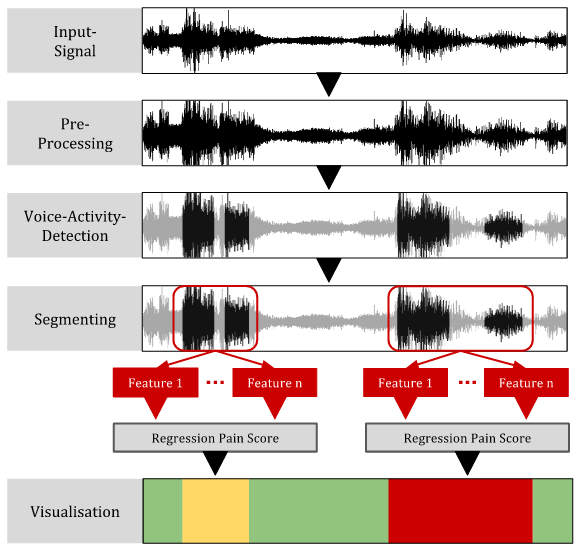
\includegraphics[width=0.75\textwidth]{bilder/pipeline01.png}
	\caption{Überblick über die Verarbeitungs-Pipeline dieser Arbeit}
	\label{img:architecture-overview}
\end{figure}